%%%%%%%%%%%%%%%%%%%%%%%%%%%%%%%%%%%%%%%%%
% LaTeX Template
% http://www.LaTeXTemplates.com
%
% Original author:
% Linux and Unix Users Group at Virginia Tech Wiki 
% (https://vtluug.org/wiki/Example_LaTeX_chem_lab_report)
%
% License:
% CC BY-NC-SA 3.0 (http://creativecommons.org/licenses/by-nc-sa/3.0/)
%
%%%%%%%%%%%%%%%%%%%%%%%%%%%%%%%%%%%%%%%%%

%----------------------------------------------------------------------------------------
%	PACKAGES AND DOCUMENT CONFIGURATIONS
%----------------------------------------------------------------------------------------

\documentclass[12pt]{article}
\usepackage{geometry} % Pour passer au format A4
\geometry{hmargin=1cm, vmargin=1cm} % 

\usepackage{graphicx} % Required for including pictures
\usepackage{float} % 

%Français
\usepackage[T1]{fontenc} 
\usepackage[english,francais]{babel}
\usepackage[utf8]{inputenc}
\usepackage{eurosym}
\usepackage{lmodern}
\usepackage{url}
\usepackage{multicol}

%Maths
\usepackage{amsmath,amsfonts,amssymb,amsthm}
%\usepackage[linesnumbered, ruled, vlined]{algorithm2e}
%\SetAlFnt{\small\sffamily}

%Autres
\linespread{1} % Line spacing
\setlength\parindent{0pt} % Removes all indentation from paragraphs

\renewcommand{\labelenumi}{\alph{enumi}.} % 
\pagestyle{empty}
%----------------------------------------------------------------------------------------
%	DOCUMENT INFORMATION
%----------------------------------------------------------------------------------------
\begin{document}

%\maketitle % Insert the title, author and date

\setlength{\columnseprule}{1pt}

\textbf{Nom(s), Prénom(s) :}

\subsection*{2 - Décharge d'un condensateur dans une résistance}

\fbox{\begin{minipage}{\textwidth}
    Un circuit RC est un circuit où se trouve en série une résistance R et un condensateur de capacité C. D'après la loi des mailles : $E = Ri + u$ avec $u$ la tension au borne du condensateur qu'on allume à $t=0$ et $i = C \dfrac{du}{dt}$.

    \begin{equation*}
      \left\lbrace
      \begin{array}{ccc}
        0 &= RC\dfrac{du(t)}{dt} + u(t)\\
        u(0) &= E
      \end{array}\right.
    \end{equation*}


    Pour le moment, on se propose de résoudre le problème sans donner de valeur particulière à $R$, $C$ et $E$.
\end{minipage}}


\begin{enumerate}
\item Chercher l'ensemble des solutions $u$ de l'équation :
  $$ RC \times \dfrac{du(t)}{dt} + u(t) = 0 $$

\item Soit $u$ la solution générale de notre problème initiale.

  \begin{equation*}
    \left\lbrace
    \begin{array}{ccc}
      0 &= RC\dfrac{du(t)}{dt} + u(t)\\
      u(0) &= E
    \end{array}\right.
  \end{equation*}


  Chercher l'unique solution vérifiant la condition initiale $u(0) = E$. 
\item Tracer la fonction $u$ solution de ce problème avec $E = 12V$, $R = 10\Omega$ et $C = 0.4F$.
\end{enumerate}

\begin{figure}[H]
  \centering
  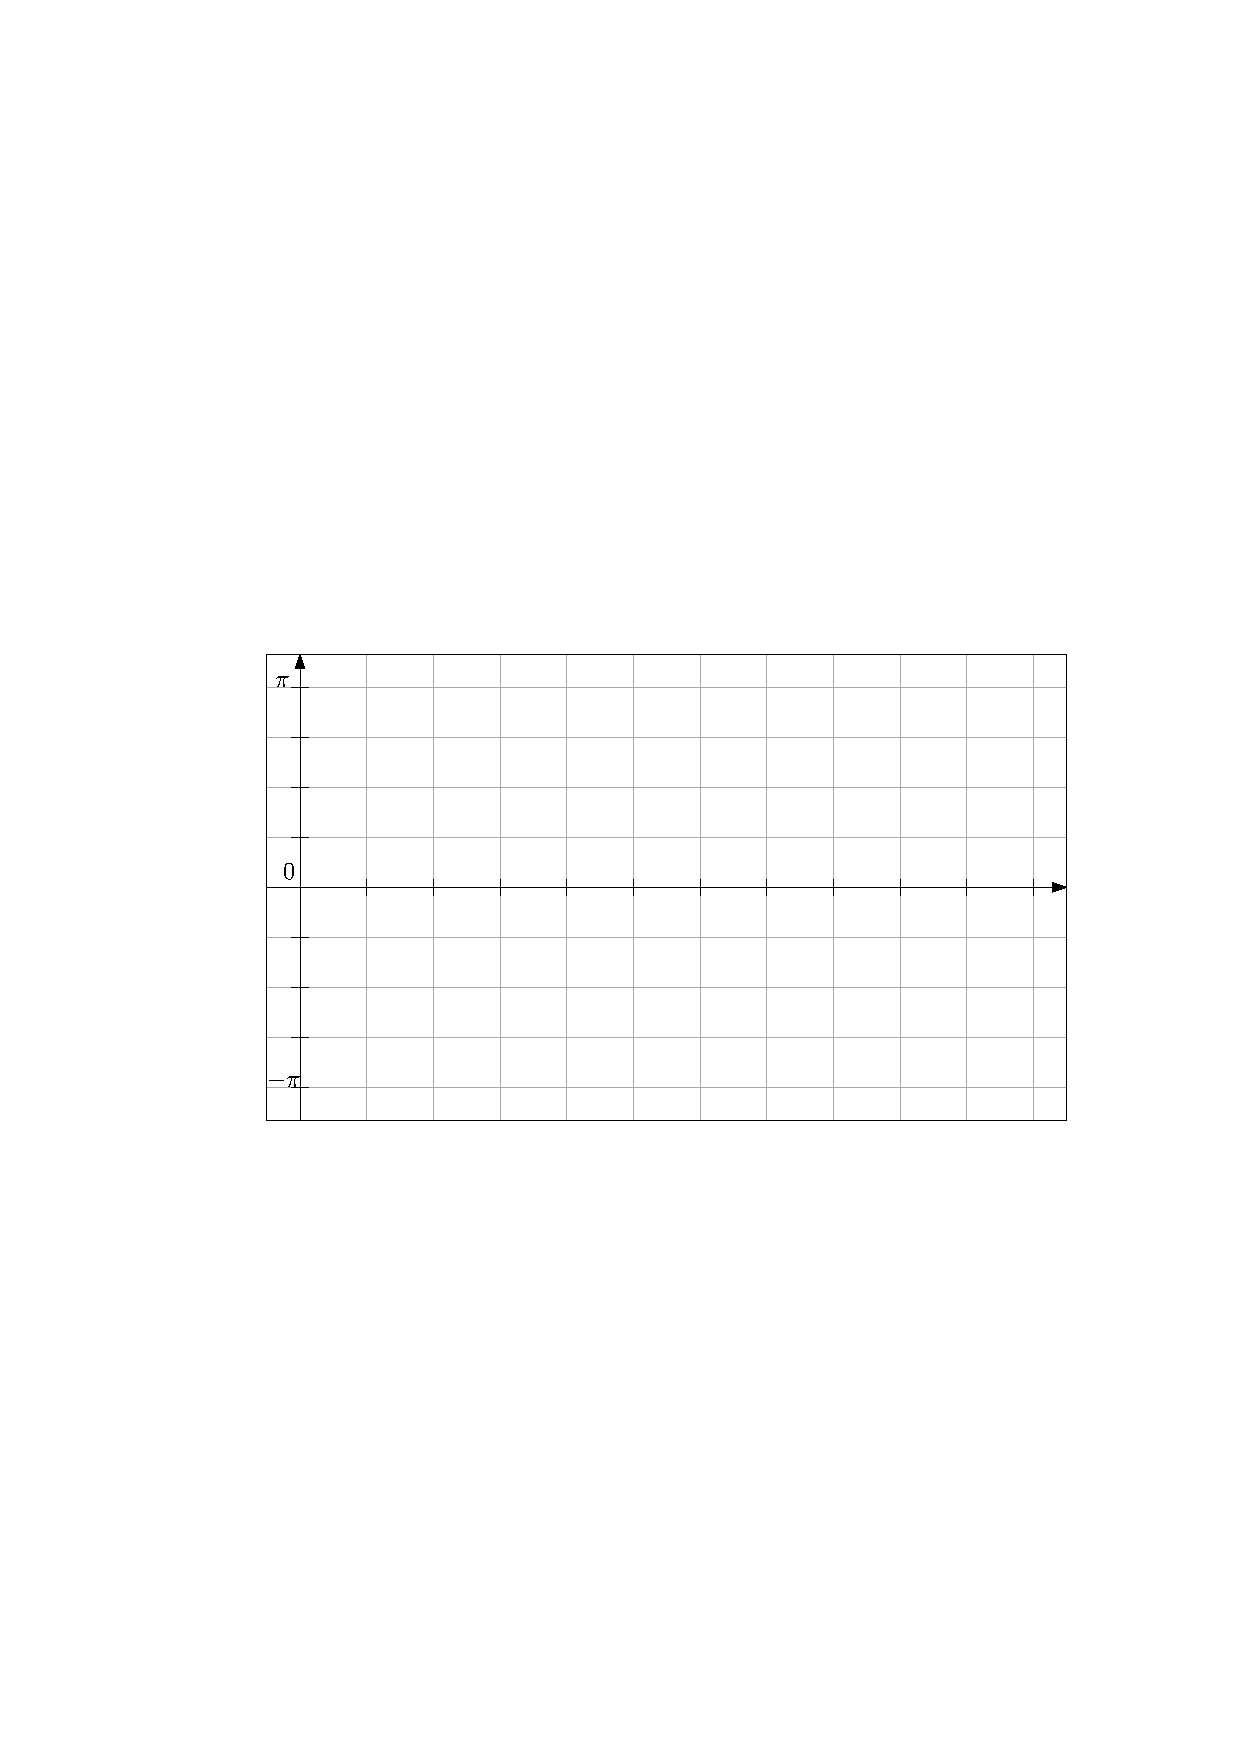
\includegraphics[width=\linewidth]{sources/2/grille.pdf}
\end{figure}

\newpage


\textbf{Nom(s), Prénom(s) :}

\subsection*{2 - Décharge d'un condensateur dans une résistance}

\fbox{\begin{minipage}{\textwidth}
    Un circuit RC est un circuit où se trouve en série une résistance R et un condensateur de capacité C. D'après la loi des mailles : $E = Ri + u$ avec $u$ la tension au borne du condensateur qu'on allume à $t=0$ et $i = C \dfrac{du}{dt}$.

    \begin{equation*}
      \left\lbrace
      \begin{array}{ccc}
        0 &= RC\dfrac{du(t)}{dt} + u(t)\\
        u(0) &= E
      \end{array}\right.
    \end{equation*}


    Pour le moment, on se propose de résoudre le problème sans donner de valeur particulière à $R$, $C$ et $E$.
\end{minipage}}


\begin{enumerate}
\item Chercher l'ensemble des solutions $u$ de l'équation :
  $$ RC \times \dfrac{du(t)}{dt} + u(t) = 0 $$

\item Soit $u$ la solution générale de notre problème initiale.

  \begin{equation*}
    \left\lbrace
    \begin{array}{ccc}
      0 &= RC\dfrac{du(t)}{dt} + u(t)\\
      u(0) &= E
    \end{array}\right.
  \end{equation*}


  Chercher l'unique solution vérifiant la condition initiale $u(0) = E$. 
\item Tracer la fonction $u$ solution de ce problème avec $E = 12V$, $R = 10\Omega$ et $C = 0.4F$.
\end{enumerate}

\begin{figure}[H]
  \centering
  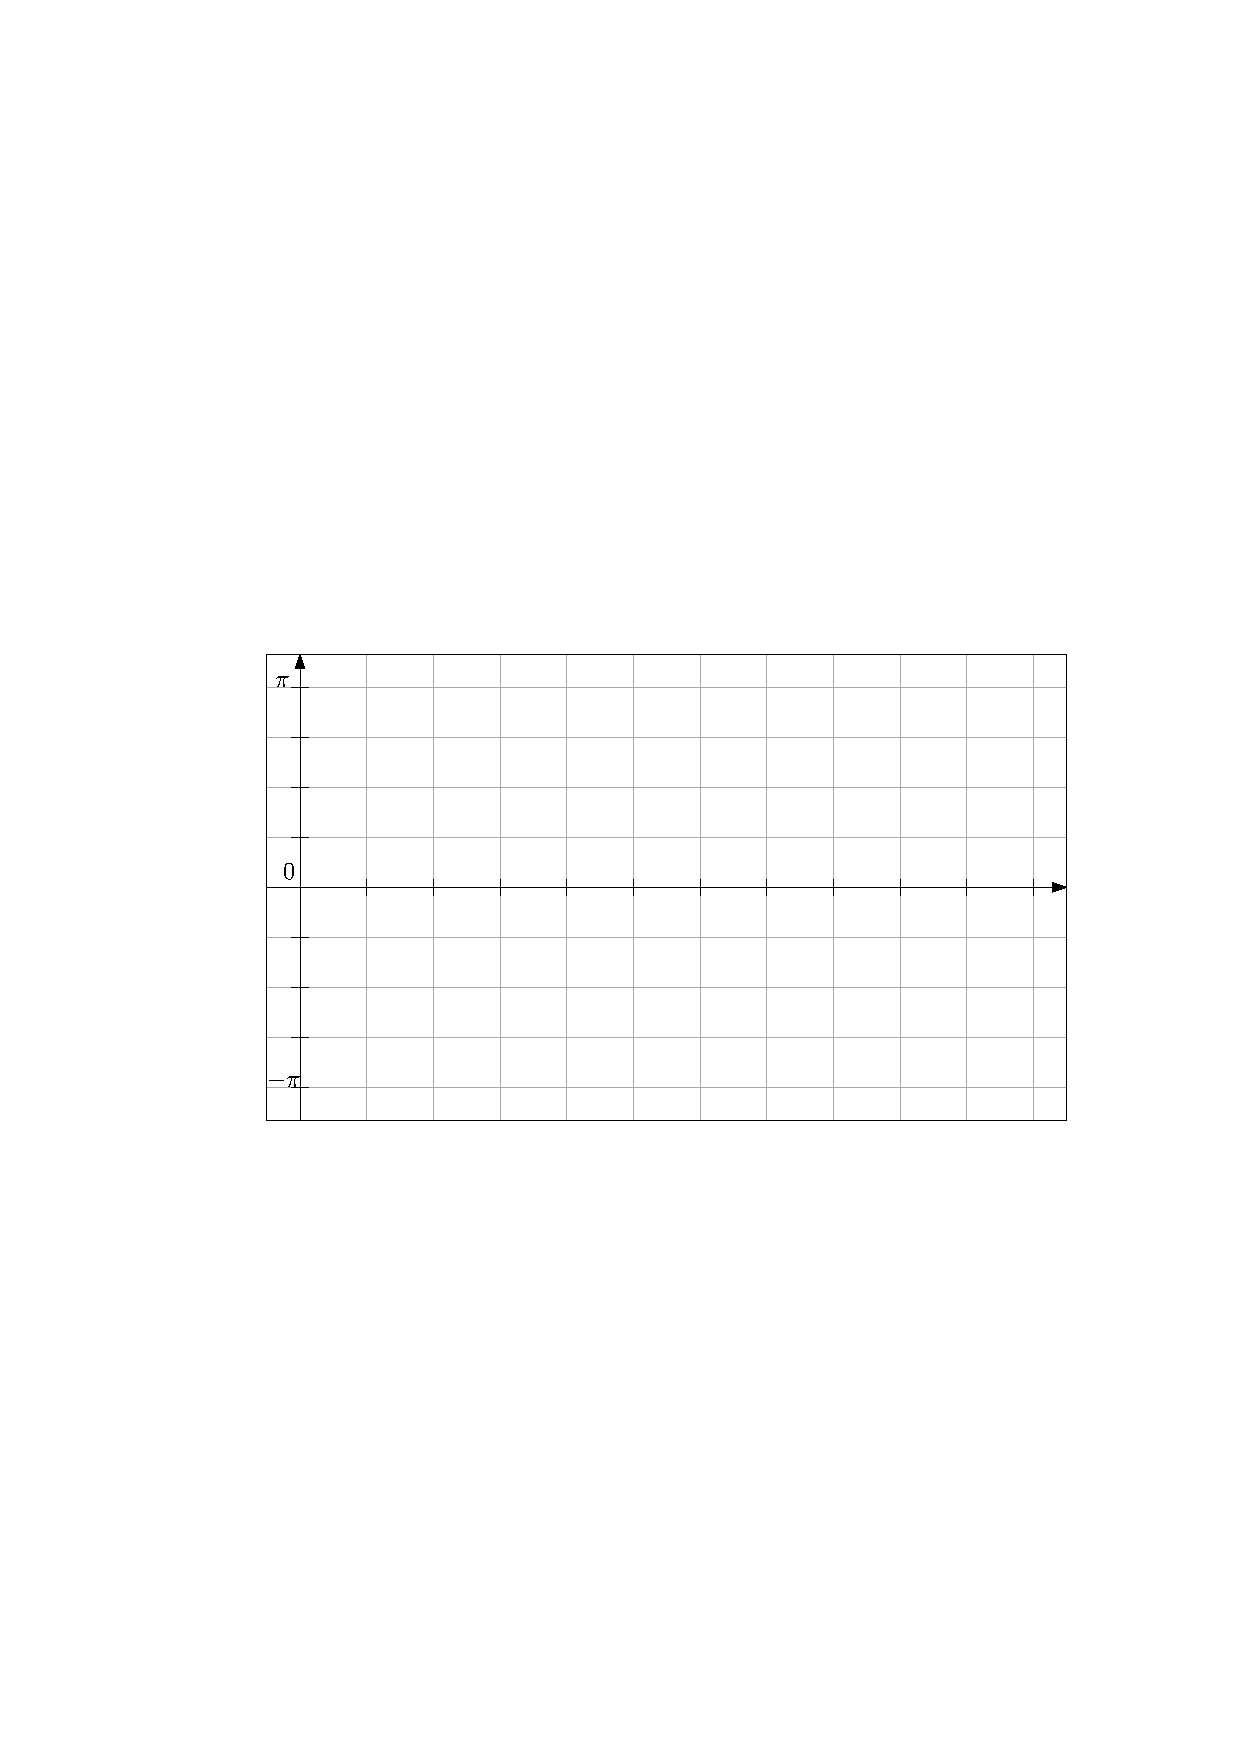
\includegraphics[width=\linewidth]{sources/2/grille.pdf}
\end{figure}


\end{document}
